\section{PACE methodology}
\label{sec:method}
Figure~\ref{fig:architecture} separates the supervised peer route from the two target-local decisions. Algorithm~\ref{alg:pace} summarizes preparation and inference; the equations below specify the score and quantile conventions.

\begin{figure}[tbp]
\centering
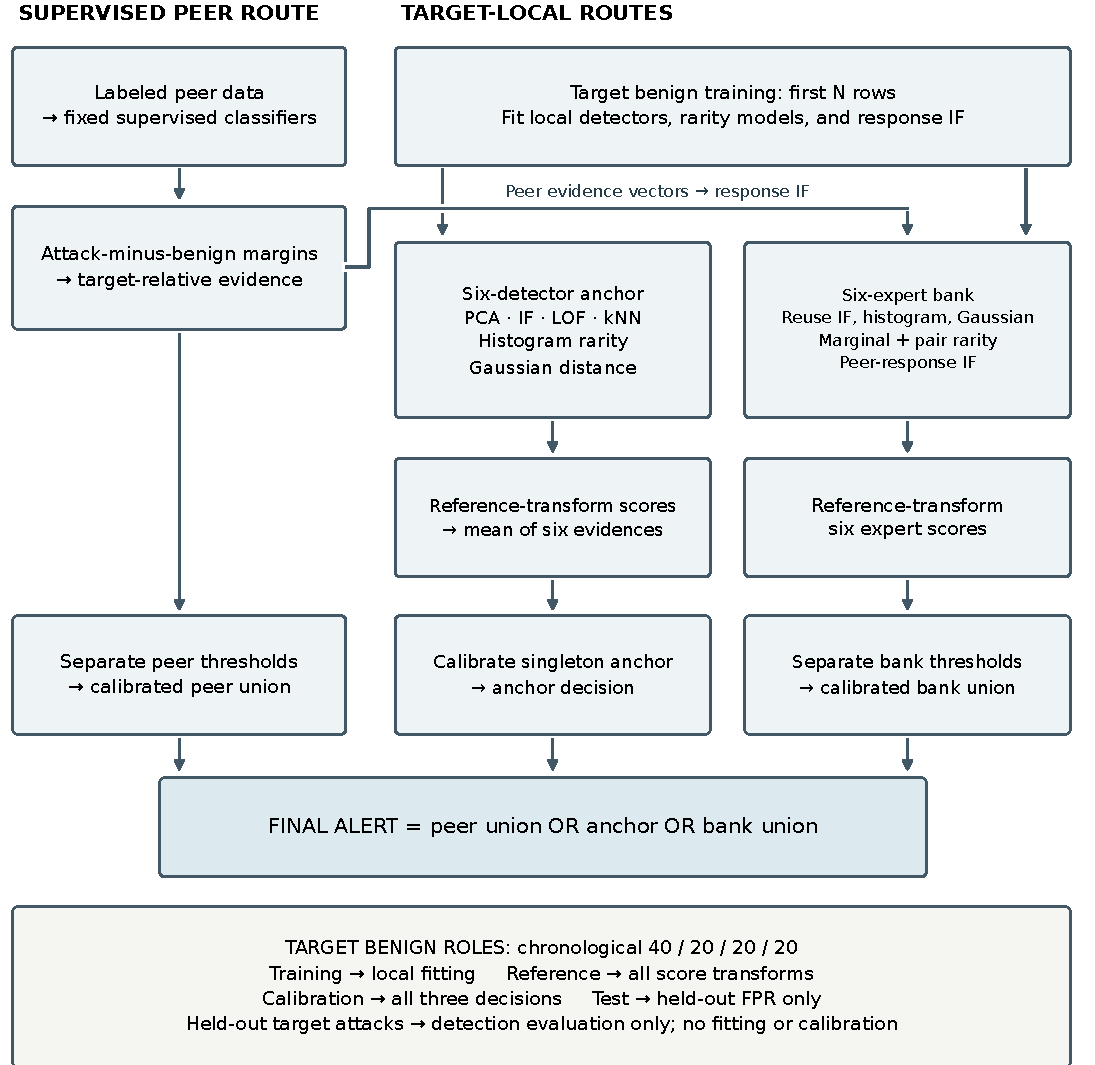
\includegraphics[width=\textwidth]{figures/architecture.pdf}
\caption{PACE's information flow and final decision. Target benign training, reference, calibration, and test roles are distinct. The benchmark standardizes features using pooled complete benign training roles before restricting local fitting to $N$ rows. Target attack labels enter evaluation only. IF: isolation forest; LOF: local outlier factor; $k$NN: nearest-neighbor distance.}
\label{fig:architecture}
\end{figure}

\subsection{Target-relative evidence}
For an expert score $s$, let $r_1,\ldots,r_n$ be that expert's scores on the target reference role, $r_{\max}=\max_i r_i$, and $d_R=\max\{r_{\max}-\operatorname{median}_i r_i,10^{-6}\}$. The implemented transformation is
\begin{equation}
 E_R(s)=\begin{cases}
 -\log\!\left(\dfrac{1+\sum_{i=1}^n\mathbf{1}\{r_i\geq s\}}{n+1}\right),&s\leq r_{\max},\\[6pt]
 \log(n+1)+\log\!\left(1+\dfrac{s-r_{\max}}{d_R}\right),&s>r_{\max}.
 \end{cases}
 \label{eq:evidence}
\end{equation}
Ties are included in the upper-tail count. Values beyond the largest reference score receive an extrapolated value, rather than a saturated empirical rank. This extrapolation is a score convention, not an estimated tail probability with a distribution-free validity guarantee. For peer $k$, the evidence is $e_k(x)=E_{R,k}(m_k(x))$.

\subsection{Blocks and thresholds}
Let $M=|C|$ and let $b=250$ be the configured block-size parameter. The code constructs $J=\max\{1,\lfloor M/b\rfloor\}$ consecutive blocks using a balanced array partition: their lengths differ by at most one, and earlier blocks receive any surplus rows. They are not necessarily blocks of exactly 250 observations. For example, 350 calibration observations form one block of length 350. Write $n_j=|C_j|$ and let $z_{j,(1)}\leq\cdots\leq z_{j,(n_j)}$ be ordered evidence in block $j$. For allocation $w\in(0,1)$,
\begin{equation}
 \tau_z(w)=\max_{1\leq j\leq J}
 z_{j,(1+\lceil(1-w)(n_j-1)\rceil)}.
 \label{eq:threshold}
\end{equation}
This is NumPy's higher empirical quantile followed by a maximum over blocks. Every decision uses a strict comparison $z(x)>\tau_z(w)$; equality does not alert. For a fixed threshold obtained this way, the observed exceedance fraction within each calibration block is at most $w$. This statement concerns the observations used to choose the threshold and does not extend to future data without additional assumptions.

\subsection{Separately calibrated experts and union scaling}
For a collection of $L$ experts with allocation $B$, the default initial shares are $w_\ell=B/L$. Given multiplier $\lambda$, the union is
\begin{equation}
 U_{B,\lambda}(x)=\mathbf{1}\!\left\{\exists\ell:
 z_\ell(x)>\tau_{z_\ell}(\lambda w_\ell)\right\}.
 \label{eq:union}
\end{equation}
The calibrator measures this union on every calibration block. Starting at $\lambda=1$, it doubles an upper search point until that point violates the block-rate criterion or reaches the allowed cap, returns immediately if the cap is feasible; otherwise it performs 20 bisections to retain a feasible lower point. The configured cap is 64. If the largest share times 64 is at least one, the implementation replaces the multiplier ceiling by $0.999/\max_\ell w_\ell$. If the initial union already violates $B$, the routine returns its initial thresholds; it does not claim to repair arbitrary supplied shares. PACE's equal-share initial unions satisfy the calibration criterion by the fixed-threshold count bound and the union bound.

The retained multiplier is a numerical search result on a stepwise calibration function. It should not be interpreted as a unique population optimum. The peer branch applies this routine to the $K$ separate margin-evidence experts with allocation $B_P$. Separate thresholds avoid collapsing all peer evidence into one maximum before calibration. The common multiplier nevertheless couples the thresholds through the observed union, so an unstable peer can still affect their joint calibration.

\subsection{Anchor and complementary local bank}
The anchor averages the reference-transformed scores of six local detectors: PCA reconstruction error, isolation forest, local outlier factor, mean nearest-neighbor distance, histogram rarity, and regularized Gaussian distance. Evidence is computed separately for each detector before averaging. The anchor is not transformed a second time. PCA retains 95\% of explained variance and uses mean squared reconstruction error. Isolation forest~\cite{liu2008isolation} uses 100 trees, local outlier factor~\cite{breunig2000lof} uses 20 neighbors, and the distance score averages 10 neighbor distances from the fitted neighbor structure. Histogram scores sum negative log smoothed bin frequencies across features, with 20 equal-width training bins and additive-one smoothing. Values outside a feature's training range use its minimum fitted bin probability. The Gaussian score is a squared Mahalanobis distance using a pseudoinverse of the sample covariance plus $0.001I$.

The local bank contains six experts. Three reuse the anchor members' isolation-forest, histogram, and Gaussian evidence. Two score feature rarity, and one scores the joint response of the peers. These feature experts reuse fitted detector outputs; they are not three additional independently fitted copies.

The first rarity expert sums two-sided empirical tail evidence. For feature $q$, let $a_q(v)$ count training values at most $v$ and $c_q(v)$ count training values strictly below $v$. Its raw score is
\begin{equation}
 s_{\mathrm{tail}}(x)=\sum_{q=1}^{d}\max\left\{
 -\log\frac{a_q(x_q)+1}{N+1},
 -\log\frac{N-c_q(x_q)+1}{N+1}\right\}.
 \label{eq:tail}
\end{equation}
This ECOD-inspired two-tail rarity score is labeled ECOD-sum in the implementation. It differs from original ECOD~\cite{ecod2022}, which maximizes three aggregate scores formed from left, right, and skewness-selected tails. Here the featurewise larger negative-log tail is selected before summation; the equation specifies the implemented variant.

For pair co-occurrence, 150 ordered feature-index pairs are drawn with replacement. Self-pairs are discarded when more than one feature is available; duplicate pairs can remain, so 150 is a draw count rather than a guaranteed count of distinct retained pairs. Each feature is coded using its unique internal training quantiles at levels $1/8,\ldots,7/8$, with left insertion at ties. Although these cut points give at most eight active codes, the implementation allocates a table of width $8+1=9$ in each dimension. If $h_{uv}(x)$ is the training count in the coded cell for retained pair $(u,v)$, the score is
\begin{equation}
 s_{\mathrm{pair}}(x)=\frac{1}{|\mathcal P|}\sum_{(u,v)\in\mathcal P}
 -\log\frac{h_{uv}(x)+0.5}{N+0.5\times9^2}.
 \label{eq:pair}
\end{equation}
The reference transformation in Eq.~\eqref{eq:evidence} is applied to both rarity scores.

The response expert fits a 100-tree isolation forest to vectors $\rho(x)=(e_1(x),\ldots,e_K(x))$ for $x\in T_N$. It uses the negative forest score as its anomaly score and then applies Eq.~\eqref{eq:evidence} relative to its scores on $R$. Thus it models how the collection of foreign classifiers responds to target benign data. It neither trains a gating network nor changes the supervised peer models.

\subsection{Resolution rule and final decision}
With anchor share $a=0.5$, the anchor allocation is
\begin{equation}
 B_A=\begin{cases}aB_L,&aB_L\geq1/b,\\B_L,&aB_L<1/b,\end{cases}
 \qquad B_B=(1-a)B_L.
 \label{eq:allocation}
\end{equation}
The anchor is itself calibrated by the union-scaling routine as a singleton expert with allocation $B_A$. The bank is separately calibrated as a six-expert union with allocation $B_B$. In particular, the anchor threshold is not merely the unscaled quantile $\tau_A(B_A)$. Let the resulting decisions be $U_P$, $U_A$, and $U_B$. The final rule is
\begin{equation}
 D(x)=U_P(x)\lor U_A(x)\lor U_B(x).
 \label{eq:final}
\end{equation}
There is no final calibration pass over this three-way union.

At $\alpha=0.01$ and $r=a=0.5$, these allocations are $B_P=0.005$, $B_A=0.005$, and $B_B=0.0025$. Their sum is 0.0125, rather than 0.01. At $\alpha=0.05$, they are 0.025, 0.0125, and 0.0125, whose sum is 0.05. Overlap and integer count resolution can make the observed calibration union smaller than the allocation sum, but do not justify presenting Eq.~\eqref{eq:allocation} as a strict partition of $\alpha$. The rule checks $1/b$, whereas the first possible nonzero exceedance for an individual higher quantile depends on its actual block length through $1/(n_j-1)$. The resolution rule is therefore an implemented heuristic, not an exact test of every block's quantile resolution.

The protected anchor preserves a separate local decision path but does not prove non-inferiority to the primary comparator. That comparator averages seven detector evidences, including an autoencoder omitted from the six-member anchor, and uses a different threshold procedure. Target-level regressions must be assessed empirically.

\begin{table}[tbp]
\centering
\begin{minipage}{0.96\textwidth}
\hrule\smallskip
\refstepcounter{algorithm}\textbf{Algorithm \thealgorithm. PACE preparation and inference}\label{alg:pace}
\smallskip\hrule\smallskip
\small
\textbf{Input:} fixed peer classifiers; target benign roles $T_N,R,C$; nominal $\alpha$; $r=a=0.5$; block parameter $b=250$.
\begin{enumerate}
\setlength{\itemsep}{2pt}\setlength{\parskip}{0pt}
\item Evaluate each peer's attack-minus-benign margins on $T_N,R,C$; construct reference transforms $E_{R,k}$ by Eq.~\eqref{eq:evidence}, including ties and beyond-reference extrapolation.
\item Fit the local detectors and rarity models on $T_N$, and the response IF on $(e_1,\ldots,e_K)(T_N)$. Transform each local score against its scores on $R$. Form the six-evidence mean anchor and six-expert bank.
\item Partition $C$ into $\max(1,\lfloor |C|/b\rfloor)$ balanced consecutive blocks. For each expert, use the maximum block higher quantile in Eq.~\eqref{eq:threshold}.
\item Set $B_P=(1-r)\alpha$ and $B_L=r\alpha$. Compute $B_A,B_B$ with the resolution rule in Eq.~\eqref{eq:allocation}.
\item Apply \textsc{CalibrateUnion} to the $K$ peers with $B_P$, the singleton anchor with $B_A$, and the six bank experts with $B_B$. Store all reference transforms and thresholds.
\item For a query $x$, compute the same frozen evidences. Alert if any peer exceeds its threshold, the anchor exceeds its threshold, or any bank expert exceeds its threshold. All comparisons are strict $>$; no final recalibration is applied.
\end{enumerate}
\textbf{CalibrateUnion}$(Z,B)$: initialize equal shares $w_\ell=B/L$ and thresholds at $\lambda=1$. Use cap $c=64$, replaced by $0.999/\max_\ell w_\ell$ if $64\max_\ell w_\ell\geq1$. Return the initial thresholds if their worst block union rate exceeds $B$. Otherwise test $\min(2,c)$ and double up to $c$ while feasible; return immediately if $c$ is feasible. Once an infeasible upper point is found, perform 20 bisections, retaining the feasible lower point. Return its thresholds.
\smallskip\hrule
\end{minipage}
\end{table}

\subsection{Training and computation}
Each peer classifier has two ReLU hidden layers of widths 64 and 16 and two output logits. Training uses class-balanced cross-entropy, Adam updates, eight epochs, batch size 256, and learning rate 0.001. Target-local fitting uses the first $N$ retained training rows. The feature-space isolation-forest and neighbor-based fitting sample is limited to 8000 rows; other local components have their own full-$N$ fitting operations. Fitted score references and thresholds are fixed at inference: the evaluated rule has no online update.

The benchmark's shared local ensemble also trains and scores an autoencoder for the mean-ensemble comparator, even though its score is excluded from PACE's anchor. It would therefore be inaccurate to describe the executed campaign as requiring no local neural training. The detection architecture requires $K$ peer forward evaluations plus local score computations; the response forest adds a model in $K$ dimensions. A peer MLP contains $64d+1138$ weights and biases for $d$ input features. This algebraic parameter count is not a measurement of serialization size, communication traffic, latency, energy use, or deployment memory. None of those operational quantities is established by the reported detection results.



